
\documentclass[style=sailor,size=12pt]{powerdot}
\usepackage{epic,array,ecltree,url}
\usepackage[nointegrals]{wasysym}
\usepackage{mathtools}
\usepackage{graphicx}
\graphicspath{ {../art/} }
\usepackage[labelformat=empty]{caption}

\newcommand{\id}[1]{\mbox{\it #1\/}}
\newcommand{\rid}[1]{\mbox{\rm #1}}
\newcommand{\sid}[1]{\mbox{\sf #1}}
\newcommand{\bid}[1]{\mbox{\bf #1}}
\newcommand{\tinysz}[1]{\mbox{\tiny $#1$}}

\newcommand{\lra}{\longrightarrow}
\newcommand{\ra}{\rightarrow}
\newcommand{\surj}{\twoheadrightarrow}
\newcommand{\graph}{\mathrm{graph}}
\newcommand{\bb}[1]{\mathbb{#1}}
\newcommand{\Ell}{\mathscr{L}}
\newcommand{\Z}{\bb{Z}}
\newcommand{\Q}{\bb{Q}}
\newcommand{\R}{\bb{R}}
\newcommand{\C}{\bb{C}}
\newcommand{\N}{\bb{N}}
\newcommand{\M}{\mathbf{M}}
\newcommand{\m}{\mathbf{m}}
\newcommand{\MM}{\mathscr{M}}
\newcommand{\HH}{\mathscr{H}}
\newcommand{\Om}{\Omega}
\newcommand{\Ho}{\in\HH(\Om)}
\newcommand{\bd}{\partial}
\newcommand{\del}{\partial}
\newcommand{\bardel}{\overline\partial}
\newcommand{\textdf}[1]{\textbf{\textsf{#1}}\index{#1}}
\newcommand{\img}{\mathrm{img}}
\newcommand{\ip}[2]{\left\langle{#1},{#2}\right\rangle}
\newcommand{\inter}[1]{\mathrm{int}{#1}}
\newcommand{\exter}[1]{\mathrm{ext}{#1}}
\newcommand{\cl}[1]{\mathrm{cl}{#1}}
\newcommand{\ds}{\displaystyle}
\newcommand{\vol}{\mathrm{vol}}
\newcommand{\cnt}{\mathrm{ct}}
\newcommand{\osc}{\mathrm{osc}}
\newcommand{\LL}{\mathbf{L}}
\newcommand{\UU}{\mathbf{U}}
\newcommand{\support}{\mathrm{support}}
\newcommand{\AND}{\;\wedge\;}
\newcommand{\OR}{\;\vee\;}
\newcommand{\Oset}{\varnothing}
\newcommand{\st}{\ni}
\newcommand{\wh}{\widehat}
\newcommand{\mli}[1]{\mathit{#1}}
\newcommand{\ndiv}{\hspace{-3pt}\not|\hspace{2pt}}

\newcommand{\node}{%
  \begingroup\normalfont
  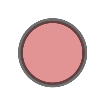
\includegraphics[height=\fontcharht\font`\c]{node.eps}%
  \endgroup
}

\newcommand{\twonode}{%
  \begingroup\normalfont
  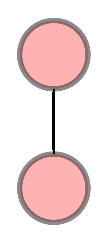
\includegraphics[height=\fontcharht\font`\b]{2nodetree.eps}%
  \endgroup
}
\newcommand{\threenode}{%
  \begingroup\normalfont
  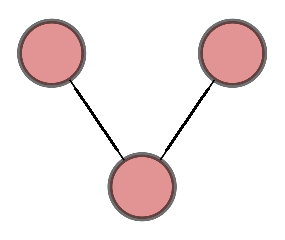
\includegraphics[height=\fontcharht\font`\b]{3nodetree.eps}%
  \endgroup
}

\pdsetup{method=normal,
list={labelsep=1em,leftmargin=1cm,itemsep=0pt,topsep=5pt,parsep=0pt}
}
% import from truth and PTL.
\title{Sample Derivations Step-by-Step}
\author{Foundations of Computer Science}
\date{\today}


\begin{document}
\maketitle

\begin{wideslide}[bm=,toc=]{Recursive definitions:Positive Multiples of Three}
\begin{itemize}
\item A Post system of two productions:
\vspace{-1em}
\begin{tabbing}
{\bf R}XX \=  \kill
{\bf B} \>
        \(\begin{array}[t]{l}
        3\in S
        \end{array}\) \\[2ex]
{\bf R} \>
        \(\begin{array}[t]{l}
        x \in S \;\;\;y \in S \\
        \hline
        x + y \in S
        \end{array}\)
\end{tabbing}
\item The set of signs is $\{3,\in,+\}$ and variables $\{x,y\}$.
\item Claim: system defines the set of all positive multiples of 3.
\item Must prove $n\in S$ iff $n$ is a positive multiple of 3.
\item ``$n\in S$ only if $n$ is a positive multiple of 3'' (system {\em soundness\/}).
\item ``$n\in S$ if $n$ is a positive multiple of 3'' (system {\em completeness\/}).
\end{itemize}
\end{wideslide}

\begin{wideslide}[bm=,toc=]{Example derivation showing $9 \in S$}
\begin{center}
\begin{tabular}{lllll}
  \onslide{2-}{$\bid{B}$  & $\id{3}\in \id{S}$}           & \onslide{3-}{$\id{3}\in \id{S}$ & $\bid{B}$}
  \onslide{4-}{\\ \cline{2-3}}
  \onslide{5-}{$\bid{R}$  & $\id{3} + \id{3} \in \id{S}$} &                    & \onslide{6-}{$\id{3}\in \id{S}$ & $\bid{B}$} 
  \onslide{7-}{\\ \cline{2-4}} 
  \onslide{8-}{$\bid{R}$  & $\id{3} + \id{3} + \id{3} \in \id{S}$ &           & &  \\} 
\end{tabular}
\end{center}

\end{wideslide}

\begin{wideslide}[bm=,toc=]{Rooted trees in Rosen 7th Ed.}
  Recall the definition of rooted trees given in Rosen (p. 351).
  
  The set of \emph{rooted trees}, where a rooted tree consists of a set of
  vertices containing a distinguished vertex called the \emph{root}, and
  edges connecting these vertices, can be defined recursively by these steps:
  
  \begin{tabbing}
  {\bf RECURSIVE}XX \=  \kill
  {\bf BASIS} \>
           A single vertex $r$ is a rooted tree.\\[2ex]
  {\bf RECURSIVE} \>
          Suppose that $T_1,T_2,...,T_n$ are disjoint rooted trees with roots\\
  {\bf } \>
          $r_1,r_2,...r_n$, respectively. Then the graph formed by starting with\\
  {\bf } \>
          a root $r$, which is not in any of the rooted trees $T_1,T_2,...T_n$,\\
  {\bf } \>
          and adding an edge from $r$ to each of the vertices $r_1,r_2,...r_n$, \\
  {\bf } \>
          is also a rooted tree.\\[2ex] \\
\end{tabbing}
\end{wideslide}

\begin{wideslide}[bm=,toc=]{Rooted trees}
\begin{itemize}
\item We want a definition amenable to induction---use a Post system instead.
\item Need 3 {\em constructors\/} $\id{cons}$, $\id{node}$ and $\id{nil}$.

\vspace{1em}
\begin{tabular}{|ll|} \hline
{\em integer list\/} & {\em list shorthand} \\ \hline
$\id{nil}$ & $[\;]$ \\
$\id{cons}(3,\id{nil})$ & $[3]$ \\
$\id{cons}(5,\id{cons}(3,\id{nil}))$ & $[5,3]$ \\
$\id{cons}(2,\id{cons}(5,\id{cons}(3,\id{nil})))$ & $[2,5,3]$ \\ \hline
\end{tabular}

\vspace{1em}
\begin{tabular}{|ll|} \hline
{\em rooted tree list: \/}$l$ & {\em rooted tree}: $t = \id{node}(l)$  \\ \hline
$l = \id{nil}$ & $\id{node}(\id{nil}) = $ \node \\
$l = \id{cons}(\id{node}(\id{nil}), \id{nil})$ & $\id{node}([\node]) = \twonode $ \\
$l = \id{cons}(\id{node}(\id{nil}),\id{cons}(\id{node}(\id{nil}),\id{nil}))$ &
$\id{node}([\node,\node]) = \threenode$ \\ \hline
\end{tabular}
\vspace{1em}
\item Let {\em RT\/} be the set of rooted trees.
%\item A list of rooted trees is a finite list of elements of RT ($t_1,t_2...t_n$).
\item Let {\em RTL\/} be the set of all lists of rooted trees.
\end{itemize}
\end{wideslide}

\begin{wideslide}[bm=,toc=]{Recursive definitions: Rooted Trees}
\begin{itemize}
\item A mutually-recursive definition of {\em rooted trees\/}:
\vspace{-1em}
\begin{tabbing}
{\bf R1}XX \=  \kill
{\bf B} \>
        \(\begin{array}[t]{l}
        \id{nil}\in\id{RTL}
        \end{array}\) \\[2ex]
{\bf R1} \>
        \(\begin{array}[t]{l}
        t\in\id{RT}\;\;\;l\in\id{RTL} \\
        \hline
        \id{cons}(t,l)\in\id{RTL}
        \end{array}\) \\[2ex]
{\bf R2} \>
        \(\begin{array}[t]{l}
        l\in\id{RTL} \\
        \hline
        \id{node}(l)\in\id{RT}
        \end{array}\)
\end{tabbing}
\item Compare with definition in Rosen 7th Ed.
\item Rosen ignores mutual recursion and hence mutual induction.
\item His definition is not induction friendly.
\end{itemize}
\end{wideslide}

\begin{wideslide}[bm=,toc=]{Sample RT derivation}
\begin{center}
\begin{tabular}{llllll}
  \onslide{2-}{             &                                 & $\bid{B}$ & $\id{nil}\in\id{RTL}$           &                       &} 
  \onslide{3-}{\\ \cline{4-4}} 
  \onslide{4-}{$\bid{B}$  & $\id{nil}\in\id{RTL}$}
  &\onslide{3-}{$\bid{R2}$             & $\id{node}(\id{nil})\in\id{RT}$} & \onslide{4-}{$\id{nil}\in\id{RTL}$ & $\bid{B}$} 
  \onslide{5-}{\\ \cline{2-2} \cline{4-5}}
  \onslide{6-}{$\bid{R2}$ & $\id{node}(\id{nil})\in\id{RT}$} & \onslide{7-}{$\bid{R1}$ & \multicolumn{2}{l}{ $\id{cons}(\id{node}(\id{nil}),\id{nil})\in\id{RTL}$} &} 
  \onslide{8-}{\\ \cline{2-5}}
  \onslide{9-}{$\bid{R1}$ & \multicolumn{4}{l}{$\id{cons}(\id{node}(\id{nil}),\id{cons}(\id{node}(\id{nil}),\id{nil}))
      \in \id{RTL}$}} 
  \onslide{10-}{ \\ \cline{2-5}}
  \onslide{11-}{$\bid{R2}$ & \multicolumn{4}{l}{$\id{node}(\id{cons}(\id{node}(\id{nil}),\id{cons}(\id{node}(\id{nil}),\id{nil})))\in\id{RT}$}}
\end{tabular}
\end{center}
\twocolumn[
lfrprop={},
lineheight=2cm,topsep=0.3cm
]{Rooted Tree Lists \\ \vspace{1mm}\hrule \vspace{1mm} 
    \onslide{2-}{[]}\\
    \onslide{7-}{[\node]}\\ 
    \onslide{9-}{[\node,\node]}
}{Rooted Trees \\ \vspace{1mm}\hrule \vspace{1mm} 
  \onslide{3-}{\node}\\ 
  \onslide{11}{\threenode}}
%\begin{figure}[h]
%\centering
%\includegraphics[width=2.5in, height=.75in,keepaspectratio=true]{3_node_tree.eps}
%\caption{3 node rooted tree derived above}
%\label{2sp}
%\end{figure}
\end{wideslide}





\end{document}
